\section{Simulation Analysis}
\label{sec:simulation}
It’s important to mention that the node $V_4$, $V_5$, $V_6$ and $V_7$, from the simulation, correspond respectively to the nodes $V_5$, $V_6$, $V_7$ and $V_8$ from the theoretical part and, the node 8 has the same voltage and current as the node 6 of the simulation, due to the existence of a null voltage source, used to measure that current that passes through those two nodes. Besides this, there’s an extra node in the simulation, which is the node 8 mentioned earlier.

\subsection{Operating point Analysis (for t<0 and Vs(t) = 0)}

Ngspice was used to perform an operating point analysis for t<0 (obtaining the table below) and by setting $v_s = 0$ and replacing the capacitor with a voltage sorce $V_x = V_6 - V_8$, the voltage and current values, present in tables below, were obtained.

\begin{table}[h!]
	\centering
	\begin{tabular}{|l|r|}
		\hline    
		{\bf Name} & {\bf Value [mA]} \\ \hline
		@c[i] & 0.000000e+00\\ \hline
@g1[i] & -2.54235e-04\\ \hline
@r1[i] & 2.428134e-04\\ \hline
@r2[i] & -2.54235e-04\\ \hline
@r3[i] & -1.14215e-05\\ \hline
@r4[i] & 1.174094e-03\\ \hline
@r5[i] & -2.54235e-04\\ \hline
@r6[i] & 9.312805e-04\\ \hline
@r7[i] & 9.312805e-04\\ \hline
v(1) & 5.026261e+00\\ \hline
v(2) & 4.779742e+00\\ \hline
v(3) & 4.248216e+00\\ \hline
v(4) & 4.815245e+00\\ \hline
v(5) & 5.586461e+00\\ \hline
v(6) & -1.87151e+00\\ \hline
v(7) & -2.80798e+00\\ \hline
v(8) & -1.87151e+00\\ \hline

	\end{tabular}
	\caption{Current and voltage results obtained with Ngspice for t<0 }
	\label{tab:op}
\end{table}



\begin{table}[h!]
	\centering
	\begin{tabular}{|l|r|}
		\hline    
		{\bf Name} & {\bf Value [mA]} \\ \hline
		@g1[i] & 2.140176e-18\\ \hline
@r1[i] & -2.04403e-18\\ \hline
@r2[i] & 2.140176e-18\\ \hline
@r3[i] & 9.614768e-20\\ \hline
@r4[i] & 4.331265e-19\\ \hline
@r5[i] & -2.76726e-03\\ \hline
@r6[i] & 4.336809e-19\\ \hline
@r7[i] & 8.998149e-19\\ \hline
v(1) & 0.000000e+00\\ \hline
v(2) & 2.075218e-15\\ \hline
v(3) & 6.549660e-15\\ \hline
v(4) & 1.776357e-15\\ \hline
v(5) & 8.394437e+00\\ \hline
v(6) & -8.71527e-16\\ \hline
v(7) & -1.77636e-15\\ \hline
v(8) & -8.71527e-16\\ \hline

	\end{tabular}
	\caption{Current and voltage results obtained with Ngspice for Vs = 0}
	\label{tab:op}
\end{table}


\subsection{Transient Analysis - Natural Response}

The first step in order to compute the natural response of $v_6$ is to set $v_s(t) = 0$ and set initial conditions so that $v_6$ and $v_s$ have the same values obtained in table 10, which ensures that in the start of the transient analysis the capacitor is fully charged. The graphic in figure 11 was obtained by executing a transient analysis, with t ranging from o to 20 ms.

By analyzing the graphic we can see a quick drop in voltage from just a little above 8 ms to 0, which is due to the fact that the capacitor is just discharging and since there are no independent voltage sources, there is no voltage being provided to $v_6$.

\begin{figure}[h!] \centering
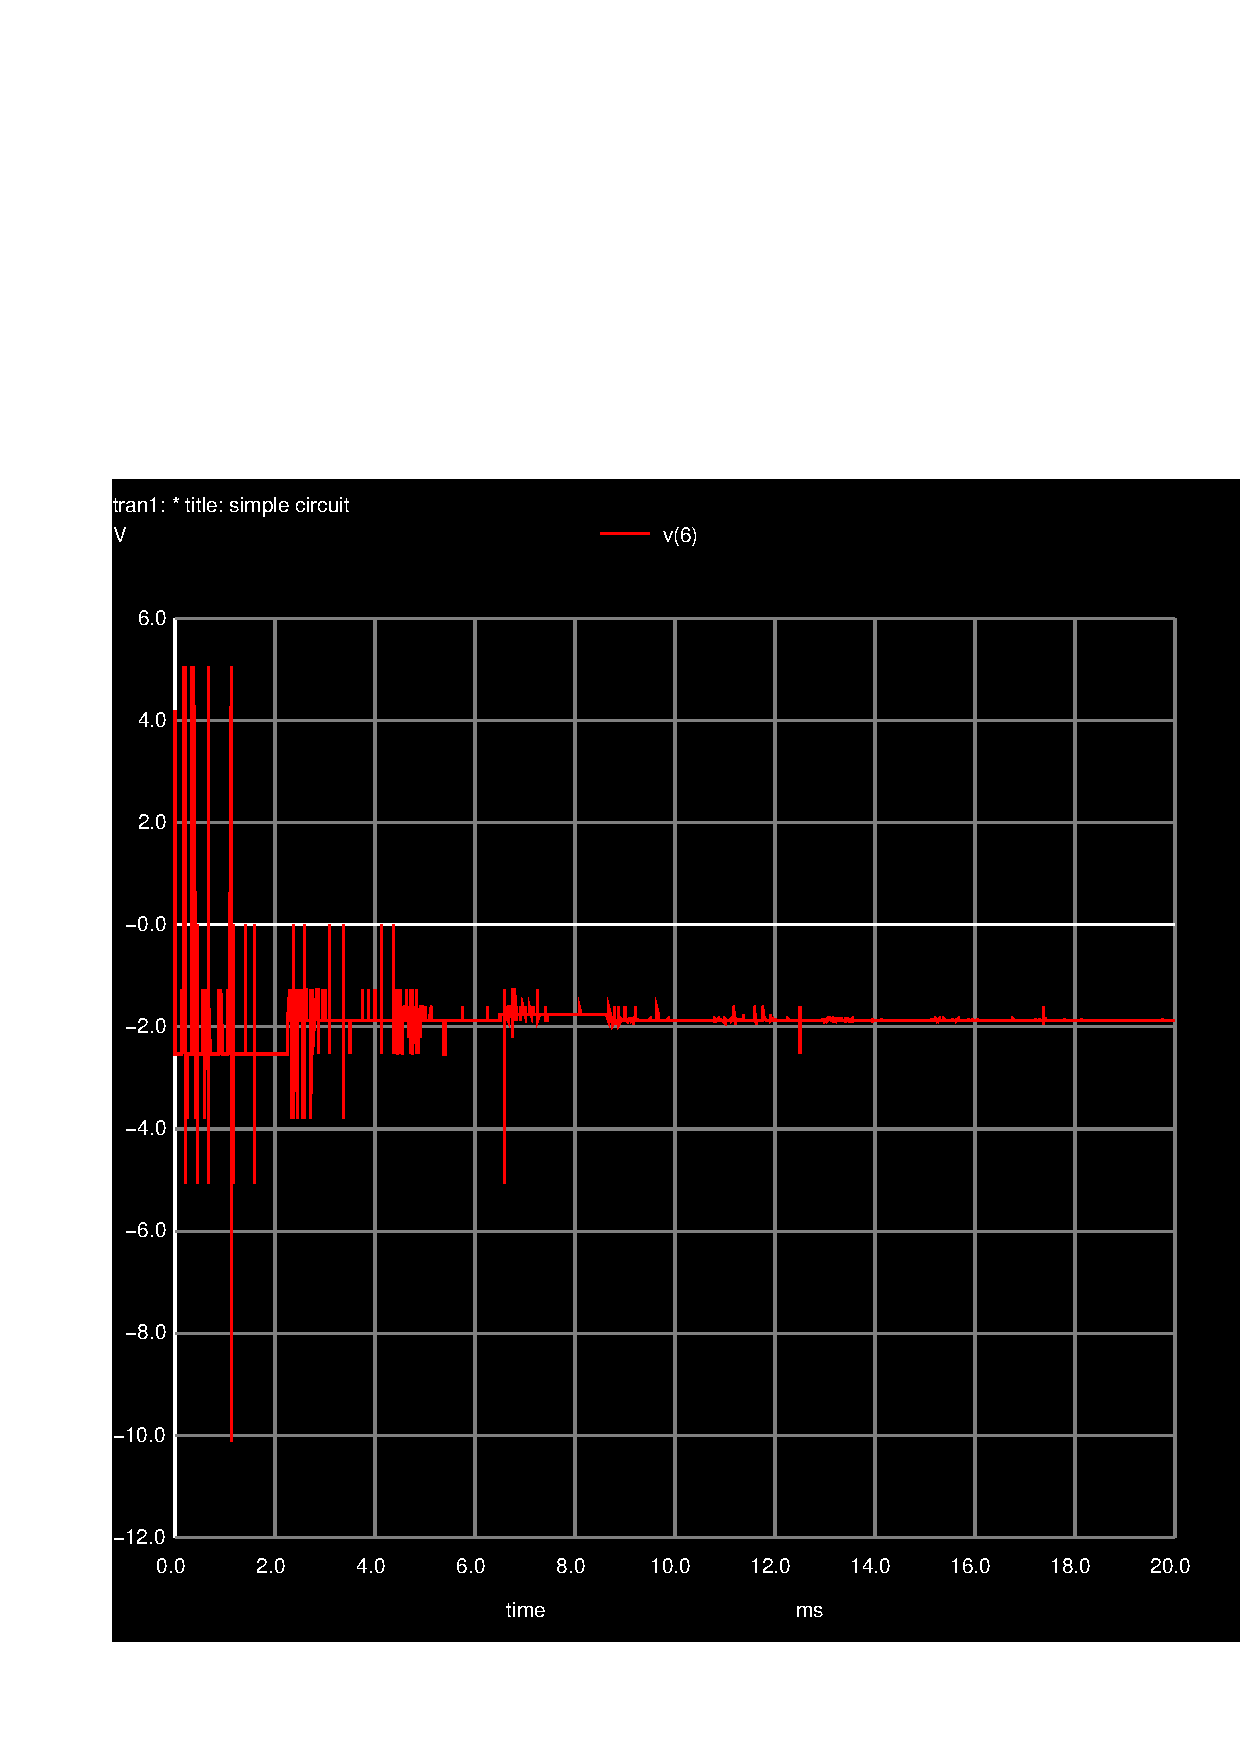
\includegraphics[width=0.6\linewidth]{trans.pdf}
\caption{Natural response}
\label{fig:rc1}
\end{figure}


\subsection{Transient Analysis - total Response}

Taking in consideration that $v_s(t) = \sin(2\pi ft)$ and f = 1000Hz, the total response can be obtained by performing a transient analysis and the figure 12 can be obtained by plotting $v_s(t)$ and $v_6(t)$. 

\begin{figure}[h!] \centering
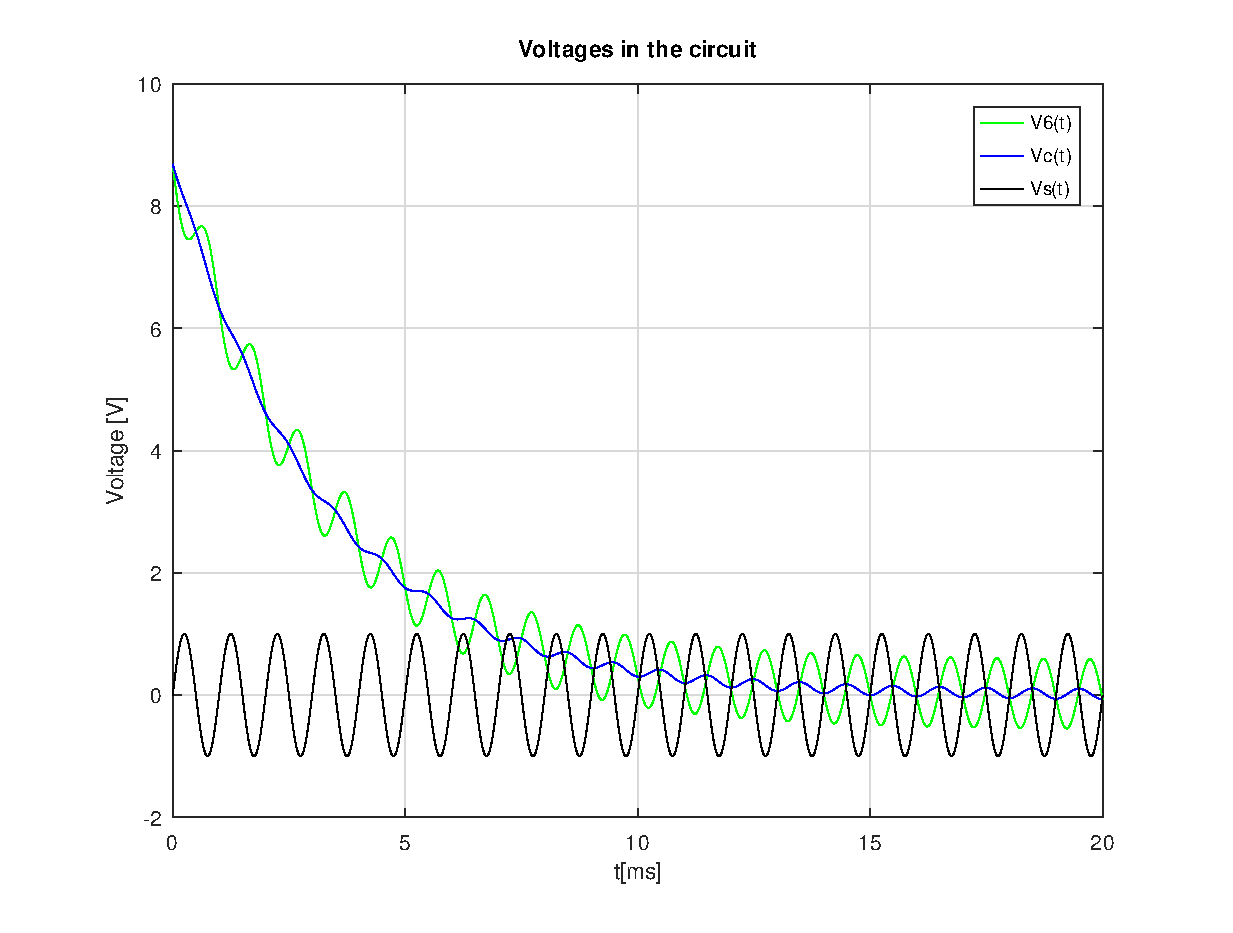
\includegraphics[width=0.6\linewidth]{global_voltage.eps}
\caption{Stinulus voltage ,$v_s(t)$, shown in black and total response, $v_6(t)$, shown in green}
\label{fig:rc1}
\end{figure}


\subsection{Frequency Response}

By excuting a frequency sweep, throughout the length of the interval [0.1, 1000000], we are able to plot the magnitude and phase, which appear below respectively.
\begin{figure}[h!] \centering
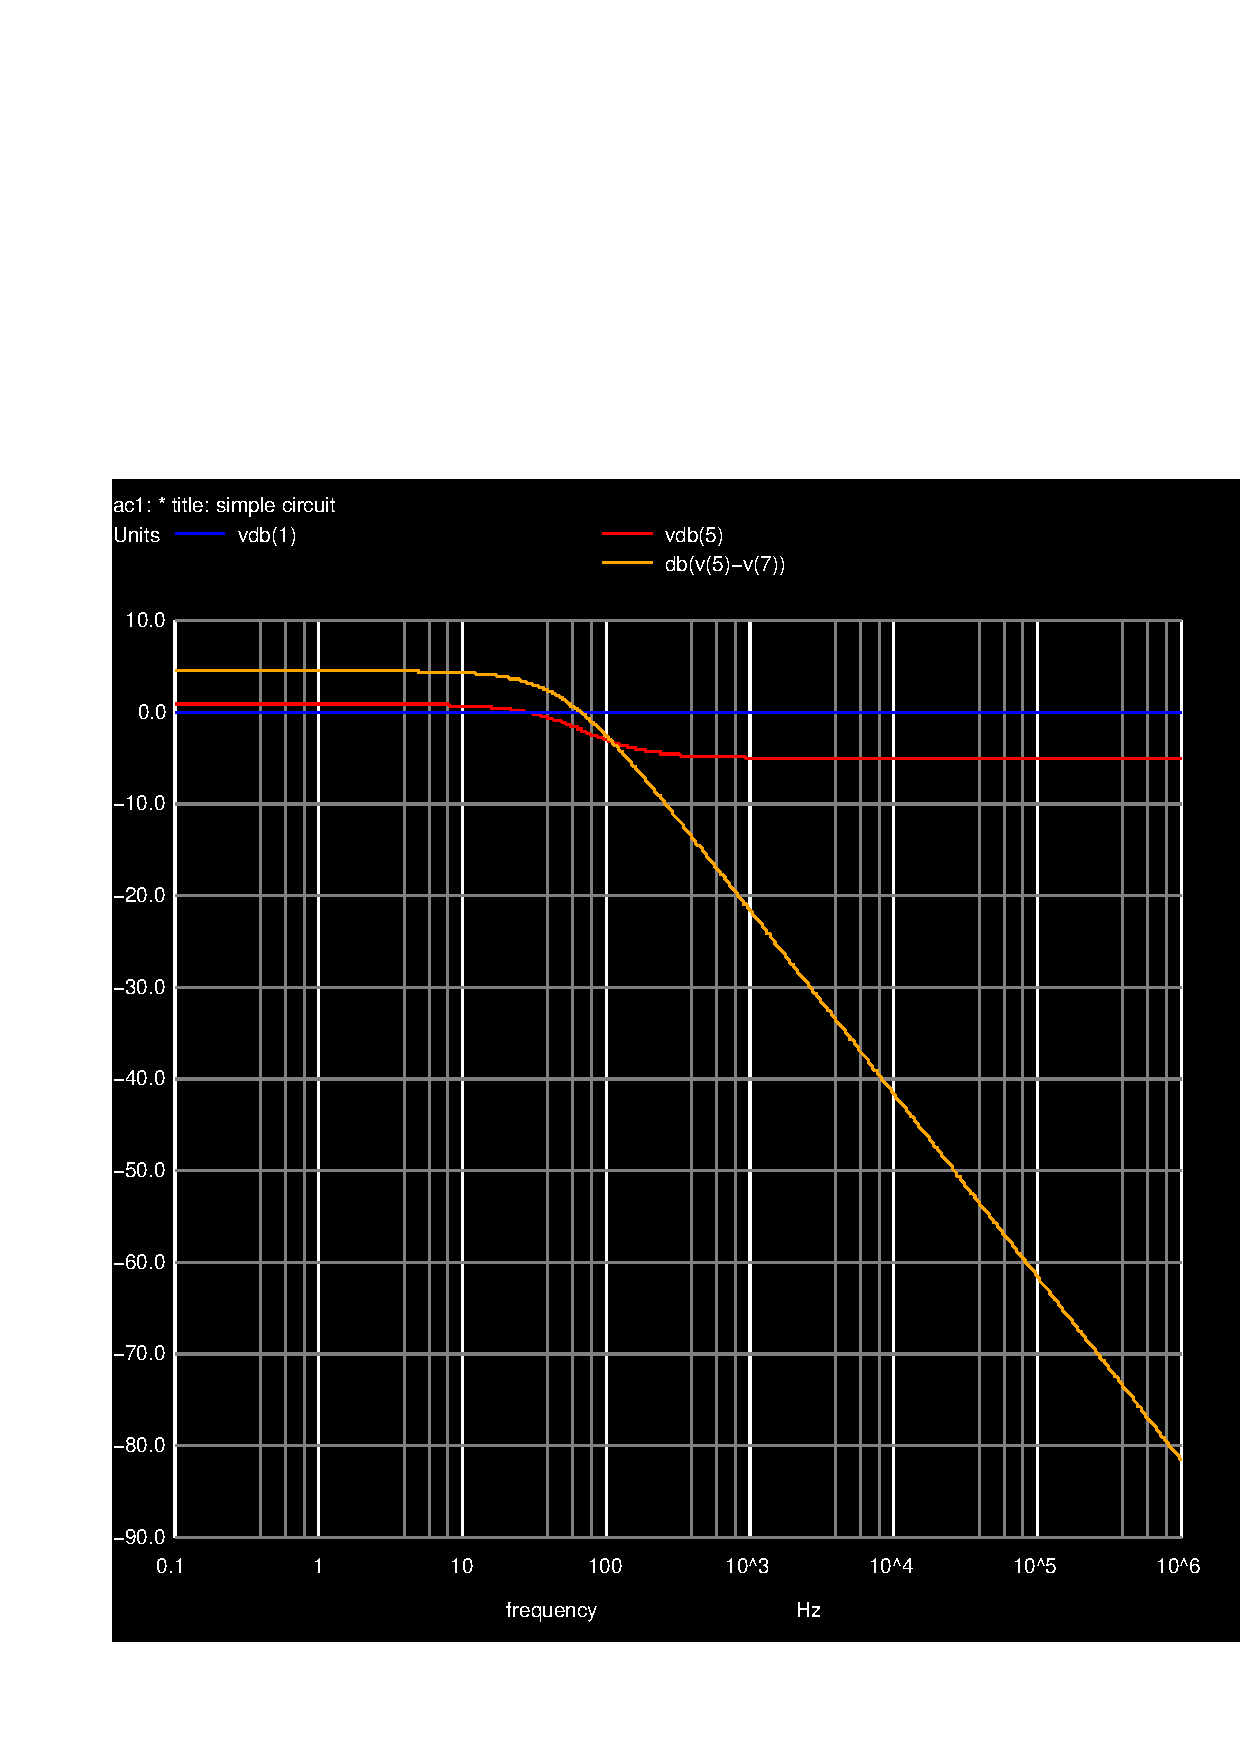
\includegraphics[width=0.6\linewidth]{acm.pdf}
\caption{Magnitude plot}
\label{fig:rc1}
\end{figure}



\begin{figure}[h!] \centering
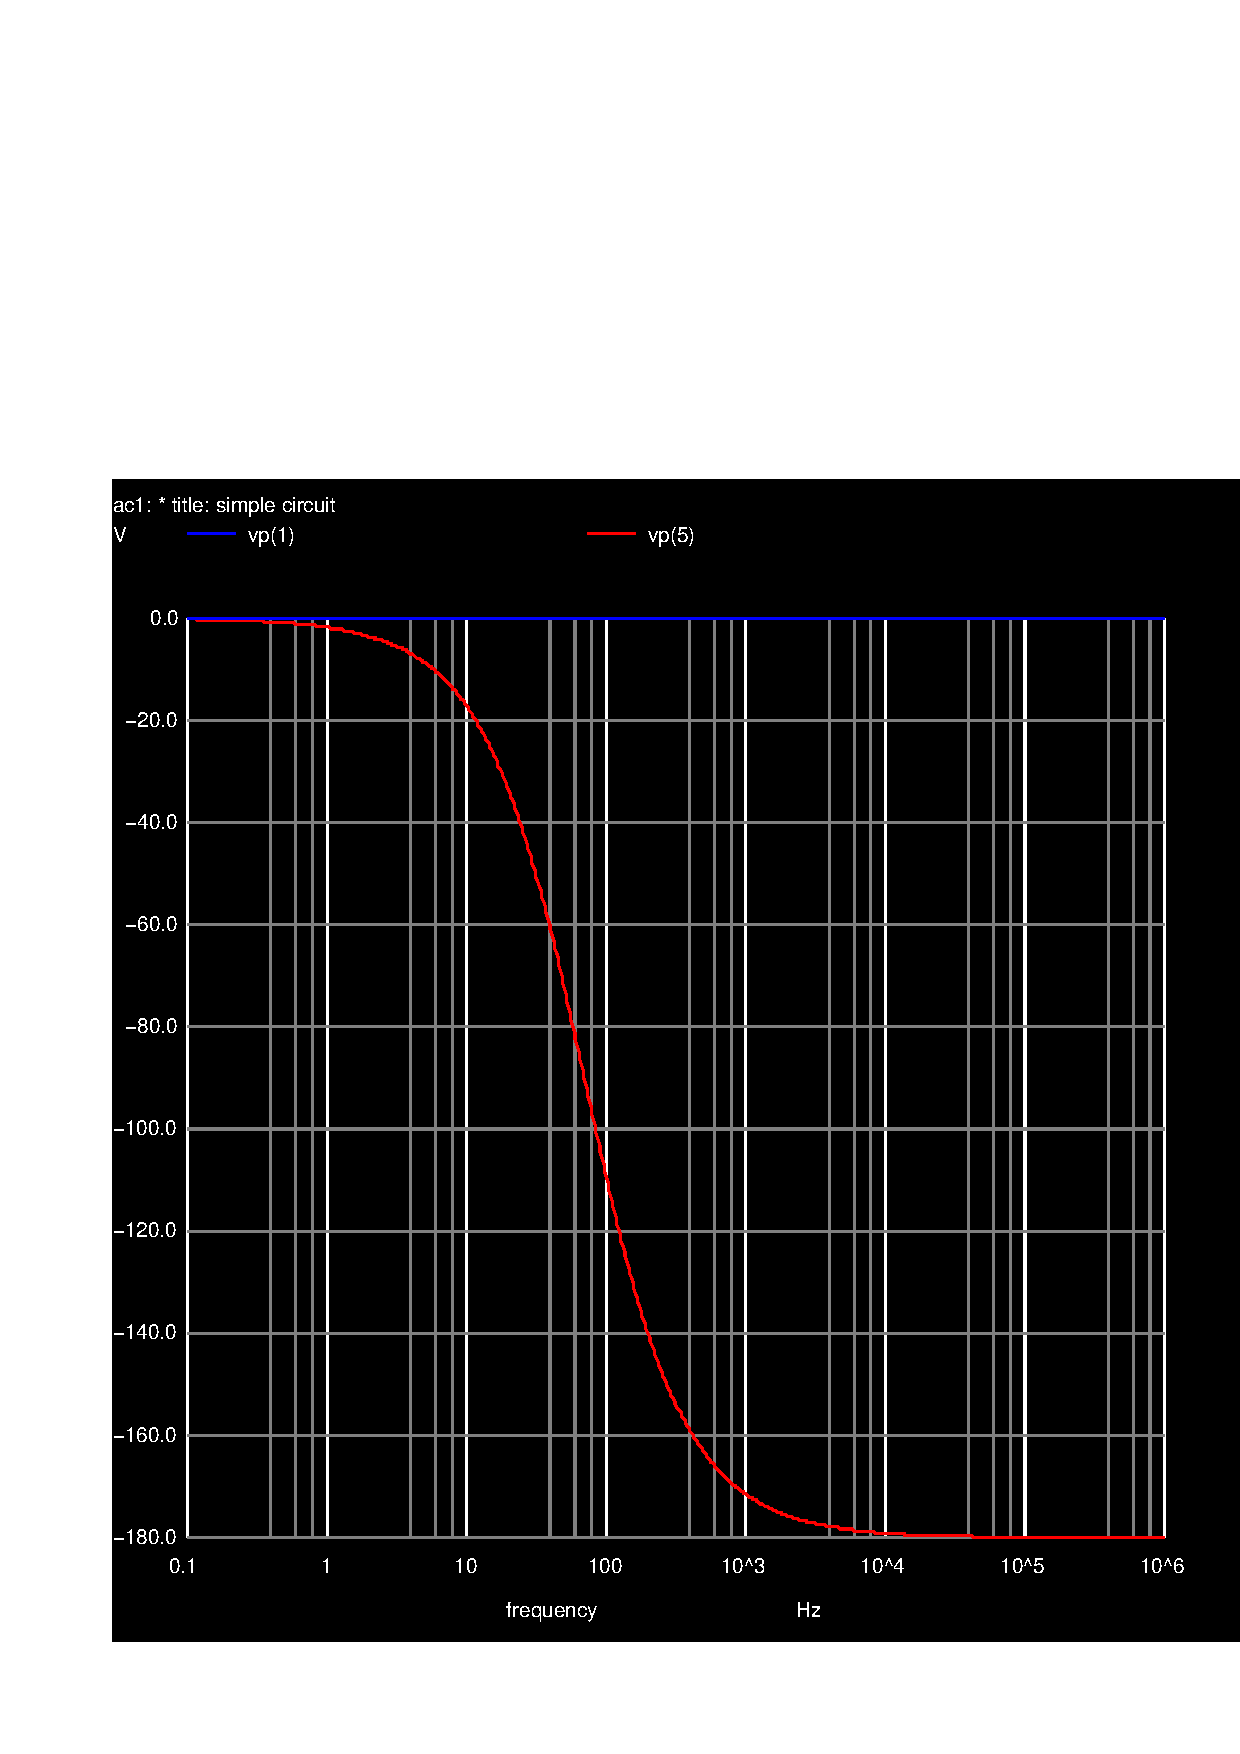
\includegraphics[width=0.6\linewidth]{acp.pdf}
\caption{Phase plot}
\label{fig:rc1}
\end{figure}

